%=============================================================================
%  Disorder in Cavity-Coupled Jahn-Teller Active Molecules
%  Beamer slide deck  --  compile with:  pdflatex present.tex   (run twice)
%
%  THEME NOTE.  This uses the built-in "Madrid" theme so it compiles with a
%  plain TeX Live install and no extra downloads.  For the sleeker look shown
%  in the plan, install the "metropolis" theme (tlmgr install beamertheme-
%  metropolis) and replace the \usetheme{Madrid} line with:
%        \usetheme{metropolis}
%  (metropolis compiles best with xelatex/lualatex).
%
%  FIGURES.  Result PNGs are pulled from ../results/ and slides/ via
%  \graphicspath below, so run pdflatex from inside the slides/ folder.
%=============================================================================
\documentclass[aspectratio=169,11pt]{beamer}

\usetheme{Madrid}
\usecolortheme{whale}
\setbeamertemplate{navigation symbols}{}
\setbeamertemplate{caption}[numbered]
\setbeamercolor{block title}{bg=structure!18,fg=black}
\setbeamercolor{block body}{bg=structure!8,fg=black}

\usepackage[utf8]{inputenc}
\usepackage[T1]{fontenc}
\usepackage{amsmath,amssymb,bm}
\usepackage{graphicx}
\usepackage{booktabs}
\usepackage{xcolor}
\usepackage{tikz}
\usetikzlibrary{arrows.meta,decorations.pathmorphing,positioning}
\usepackage[absolute,overlay]{textpos}

\graphicspath{{./}{../results/}}

% ---- bottom-of-slide source line (put a reference at the foot of a frame) ----
\newcommand{\source}[1]{%
  \begin{textblock*}{0.94\paperwidth}(0.03\paperwidth,0.905\paperheight)
    \raggedright\tiny\color{gray!75}{[Ref] #1}
  \end{textblock*}}
% ---- "our own work / code" marker (no external reference needed) ----
\newcommand{\ourcode}{%
  \begin{textblock*}{0.94\paperwidth}(0.03\paperwidth,0.905\paperheight)
    \raggedright\tiny\color{teal!70!black}{This work --- computed with our code (JT-Absorption-Spectra).}
  \end{textblock*}}

% ---- short reference strings reused across slides ----
\newcommand{\refJTa}{K. R. Nandipati \& O. Vendrell, \textit{Cavity Jahn--Teller polaritons in molecules}, Phys. Rev. A \textbf{107}, L061101 (2023).}
\newcommand{\refJTb}{S. K. Pandit, A. Pandey, A. Shankar, K. R. Nandipati, \textit{Collective Vibronic Cascade in Cavity-Coupled Jahn--Teller Active Molecules}, arXiv:2511.07880 (2025).}
\newcommand{\refArrow}{C. Dubail, T. Botzung, J. Schachenmayer, G. Pupillo, D. Hagenm\"uller, \textit{Large Random Arrowhead Matrices\ldots}, arXiv:2105.08444 (2021).}
\newcommand{\refWell}{D. Wellnitz, G. Pupillo, J. Schachenmayer, \textit{Disorder enhanced vibrational entanglement and dynamics in polaritonic chemistry}, Commun. Phys. \textbf{5}, 120 (2022).}
\newcommand{\refJahn}{H. A. Jahn \& E. Teller, Proc. R. Soc. A \textbf{161}, 220 (1937); (E$\times$e): H. C. Longuet-Higgins \textit{et al.}, Proc. R. Soc. A \textbf{244}, 1 (1958).}
\newcommand{\refEbbesen}{T. W. Ebbesen, \textit{Hybrid light--matter states\ldots}, Acc. Chem. Res. \textbf{49}, 2403 (2016).}

\title[Disorder in Cavity JT Polaritons]{Disorder in Cavity-Coupled\\ Jahn--Teller Active Molecules}
\subtitle{From single-molecule polaritons to disorder-averaged collective spectra}
\author{Summer Internship 2026}
\institute{JT-Absorption-Spectra}
\date{\today}

\begin{document}

{\setbeamertemplate{footline}{}
\begin{frame}\titlepage\end{frame}}

\begin{frame}{Outline}
  \tableofcontents
\end{frame}

%=============================================================================
\section{Cavity--matter interaction}
%=============================================================================
\begin{frame}{Molecules in an optical cavity: polaritons}
  \begin{columns}[T]
    \begin{column}{0.54\textwidth}
      \small
      \begin{itemize}
        \item A Fabry--P\'erot cavity confines the electromagnetic field to
              discrete modes of frequency $\omega_c$.
        \item When the light--matter coupling exceeds all loss rates
              (\emph{strong coupling}), molecule and photon form hybrid
              eigenstates: \textbf{polaritons}.
        \item These split into a \textbf{lower} (LP) and \textbf{upper} (UP)
              polariton, separated by the \textbf{Rabi splitting} $\Omega$.
        \item Coupling $N$ molecules collectively enhances the interaction as
              $\sqrt{N}$: the single-molecule coupling is
              $g=\Omega/(2\sqrt N)$.
        \item Polariton chemistry: modifying photophysics/reactivity by
              placing molecules in a cavity.
      \end{itemize}
    \end{column}
    \begin{column}{0.46\textwidth}
      \centering
      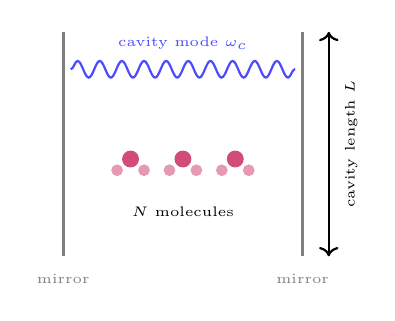
\begin{tikzpicture}[scale=0.95]
        % mirrors
        \draw[very thick,gray] (0,0) -- (0,3);
        \draw[very thick,gray] (3.2,0) -- (3.2,3);
        \node[gray] at (0,-0.3) {\tiny mirror};
        \node[gray] at (3.2,-0.3) {\tiny mirror};
        % standing wave
        \draw[blue!70,thick,decorate,decoration={snake,amplitude=3pt,segment length=8pt}]
             (0.1,2.5) -- (3.1,2.5);
        \node[blue!70] at (1.6,2.85) {\tiny cavity mode $\omega_c$};
        % molecules
        \foreach \x in {0.9,1.6,2.3}{
          \filldraw[purple!70] (\x,1.3) circle (3pt);
          \filldraw[purple!40] (\x-0.18,1.15) circle (2pt);
          \filldraw[purple!40] (\x+0.18,1.15) circle (2pt);
        }
        \node at (1.6,0.6) {\tiny $N$ molecules};
        \draw[<->,thick] (3.55,0)--(3.55,3);
        \node[rotate=90] at (3.85,1.5) {\tiny cavity length $L$};
      \end{tikzpicture}\\[0.4em]
      {\scriptsize Collective strong coupling:\\ LP/UP split by $\Omega=2\sqrt N\,g$.}
    \end{column}
  \end{columns}
  \source{\refEbbesen\ Model \& figures: \refJTb}
\end{frame}

%=============================================================================
\section{Jahn--Teller active molecules}
%=============================================================================
\begin{frame}{The Jahn--Teller effect and the $(E\times e)$ model}
  \begin{columns}[T]
    \begin{column}{0.55\textwidth}
      \small
      \textbf{Jahn--Teller theorem.} A non-linear molecule in an orbitally
      degenerate electronic state spontaneously distorts to lift the
      degeneracy.\\[0.4em]
      \textbf{$(E\times e)$ problem.} A doubly-degenerate electronic state $E$
      (components $|E_x\rangle,|E_y\rangle$) coupled to a doubly-degenerate
      vibrational mode $e$ (coordinates $Q_x,Q_y$):
      \begin{itemize}
        \item ground state $|A\rangle$, excited doublet $|E_\pm\rangle=(|E_x\rangle\pm i|E_y\rangle)/\sqrt2$;
        \item potential surfaces form a \emph{Mexican hat} with a
              \textbf{conical intersection};
        \item vibronic coupling $\kappa$ mixes electronic and nuclear motion
              $\Rightarrow$ \textbf{vibronic angular momentum} is exchanged.
      \end{itemize}
    \end{column}
    \begin{column}{0.45\textwidth}
      \centering
      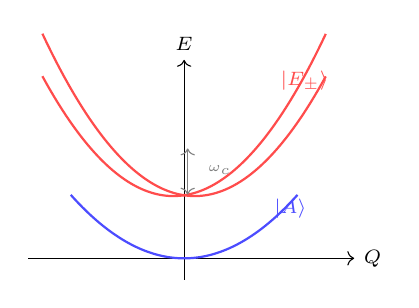
\begin{tikzpicture}[scale=0.9]
        % mexican hat cross-section
        \draw[->] (-2.2,0) -- (2.4,0) node[right]{\scriptsize $Q$};
        \draw[->] (0,-0.3) -- (0,2.8) node[above]{\scriptsize $E$};
        \draw[thick,red!70,domain=-2:2,samples=100,smooth]
          plot (\x,{0.9*(\x*\x*0.55 - 0.9) + 1.7 + 0.15*abs(\x)});
        \draw[thick,red!70,domain=-2:2,samples=100,smooth]
          plot (\x,{0.9*(\x*\x*0.55 - 0.9) + 1.7 - 0.15*abs(\x)});
        \node[red!70] at (1.7,2.5) {\scriptsize $|E_\pm\rangle$};
        % ground
        \draw[thick,blue!70,domain=-1.6:1.6,samples=80,smooth]
          plot (\x,{0.35*\x*\x});
        \node[blue!70] at (1.5,0.7) {\scriptsize $|A\rangle$};
        \draw[<->,gray] (0.05,0.9) -- (0.05,1.55);
        \node[gray] at (0.5,1.25) {\tiny $\omega_c$};
      \end{tikzpicture}\\[0.3em]
      {\scriptsize Excited $(E\times e)$ surfaces (red) and ground $|A\rangle$
      (blue) vs.\ mode coordinate $Q$.}
    \end{column}
  \end{columns}

  \begin{block}{Single-molecule JT Hamiltonian ($\hbar=1$)}
  \vspace{-0.6em}
  \[
    \hat H_{\mathrm{JT}}=\sum_{r=+,-}\big[\omega\,\hat b_r^\dagger \hat b_r
      + \epsilon\,|E_r\rangle\langle E_r|\big]
      + \kappa\big[(\hat b_+^\dagger+\hat b_-)\,|E_-\rangle\langle E_+| + \text{h.c.}\big]
  \]
  \end{block}
  \source{\refJahn\ Hamiltonian: \refJTa}
\end{frame}

%=============================================================================
\section{Single molecule: cavity Jahn--Teller polaritons (2023)}
%=============================================================================
\begin{frame}{Cavity Jahn--Teller Hamiltonian --- one molecule}
  \small
  Two perpendicular normal-incidence cavity modes ($x,y$ polarized), recast as
  circular modes $\hat a_\pm$ with angular momentum $\pm\hbar$. The
  cavity--JT Hamiltonian is
  \[
    \hat H=\hat H_{\mathrm{JT}}+\hat H_{C}+\hat H_{CM},\qquad
    \hat H_{C}=\omega_c\big(\hat a_+^\dagger \hat a_+ + \hat a_-^\dagger \hat a_-\big),
  \]
  \[
    \hat H_{CM}=\frac{\Omega}{2}\big(\hat a_+^\dagger |A\rangle\langle E_+|
      + \hat a_-^\dagger |A\rangle\langle E_-| + \text{h.c.}\big).
  \]
  \begin{columns}[T]
    \begin{column}{0.5\textwidth}
      \begin{block}{Conserved angular momentum}
      \vspace{-0.5em}
      \[ \hat J = 2\hat L_c + \hat S_z + \hat l_c \equiv 2L+s+l \]
      \vspace{-1.2em}
      \begin{itemize}\scriptsize
        \item $L_c$: vibrational pseudorotation, $S_z$: electronic, $l_c$: photon helicity.
        \item Vibronic coupling $\Rightarrow$ efficient \emph{exchange} of angular momentum between light, electrons and vibrations.
      \end{itemize}
      \end{block}
    \end{column}
    \begin{column}{0.5\textwidth}
      \begin{itemize}\scriptsize
        \item Polaritons carry \textbf{mixed $(+/-)$ circular polarization},
              set by the molecular vibronic coupling.
        \item Net cavity polarization is strongly \emph{suppressed} and becomes
              \textbf{energy dependent}.
        \item Some eigenstates show \textbf{inverted polarization}
              (opposite to the exciting field).
      \end{itemize}
    \end{column}
  \end{columns}
  \source{\refJTa}
\end{frame}

\begin{frame}{Single-molecule polaritonic spectrum (reproduced)}
  \begin{columns}[T]
    \begin{column}{0.62\textwidth}
      \centering
      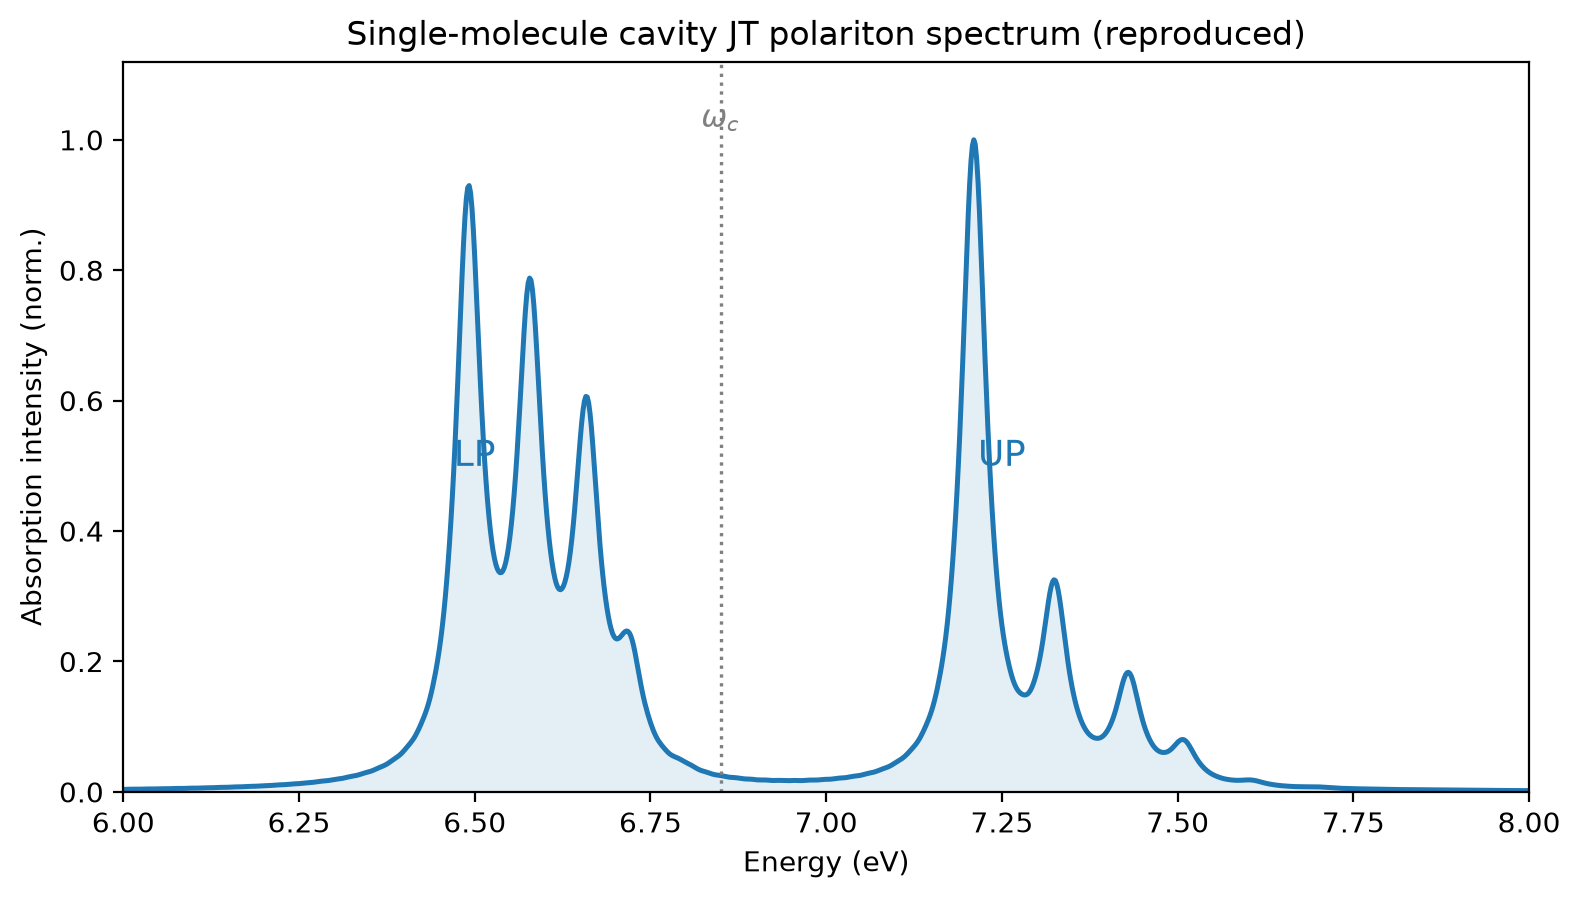
\includegraphics[width=\linewidth]{fig_repro_1mol.png}
    \end{column}
    \begin{column}{0.38\textwidth}
      \small
      \begin{itemize}
        \item Cavity set resonant with the brightest bare JT transition,
              $\omega_c=6.85$~eV.
        \item Spectrum splits into \textbf{LP} and \textbf{UP} branches, each a
              few well-resolved vibronic peaks.
        \item For $N=1$ only \textbf{3 vibronic sectors} $v\in\{0,-1,-2\}$ are
              accessible (bounded).
      \end{itemize}
      \vspace{0.5em}
      {\scriptsize Parameters: $\epsilon=7$~eV, $\omega=0.082$~eV,
      $\kappa/\omega=2.2$, $\Omega/2\omega_c=0.05$.}
    \end{column}
  \end{columns}
  \source{Physics \& parameters: \refJTa\ \ Spectrum reproduced with our code.}
\end{frame}

%=============================================================================
\section{Collective vibronic cascade (2025)}
%=============================================================================
\begin{frame}{$N$ molecules in a common cavity}
  \small
  $N$ identical JT molecules coupled to the two cavity modes:
  \[
    \hat H=\hat H_c+\sum_{k=1}^{N}\big(\hat H_{m,k}+\hat H_{m\text{-}c,k}\big),\qquad
    \hat H_{m\text{-}c,k}=\frac{\Omega}{2\sqrt N}
      \big(\hat a_+^\dagger|A\rangle\langle E_+|_k+\hat a_-^\dagger|A\rangle\langle E_-|_k+\text{h.c.}\big)
  \]
  The $\sqrt N$ normalization keeps the collective coupling
  $g=\Omega/(2\sqrt N)$ physical. Two conserved quantities:
  \begin{columns}[T]
    \begin{column}{0.5\textwidth}
      \begin{block}{Excitation number}
      \vspace{-0.6em}
      \[\hat N_{\mathrm{ex}}=\sum_k\!\big(|E_+\rangle\langle E_+|_k+|E_-\rangle\langle E_-|_k\big)+\hat a_+^\dagger\hat a_++\hat a_-^\dagger\hat a_-\]
      \end{block}
    \end{column}
    \begin{column}{0.5\textwidth}
      \begin{block}{Total angular momentum}
      \vspace{-0.6em}
      \[\hat J=\sum_{k=1}^{N}\hat V_k+\hat P,\qquad \hat V_k=2\hat L_{z,k}+\hat S_{z,k}\]
      \end{block}
    \end{column}
  \end{columns}
  \vspace{0.4em}
  We work in the optically-relevant single-excitation sector
  $(n_{\mathrm{ex}}=1,\ j=-1)$.
  \source{\refJTb}
\end{frame}

\begin{frame}{The collective vibronic cascade}
  \begin{columns}[T]
    \begin{column}{0.5\textwidth}
      \small
      Each molecule's JT Hamiltonian has vibronic eigenstates with a definite
      \textbf{vibronic angular momentum} $v=2(n_+-n_-)+S_z$:
      \[\hat H_{m,k}=\sum_v\sum_i \lambda_i^{v}\,|\lambda_i^{v}\rangle\langle\lambda_i^{v}|_k\]
      \begin{itemize}
        \item \textbf{$N=1$:} bounded --- only $v\in\{0,-1,-2\}$ reachable
              $\Rightarrow$ participation ratio $\mathrm{PR}\le 3$.
        \item \textbf{$N\ge 2$:} the cavity photon shuttles angular momentum
              \emph{between} molecules $\Rightarrow$ an unbounded ladder of $v$
              sectors --- the \textbf{collective vibronic cascade}.
      \end{itemize}
      \vspace{0.3em}
      Cascade metric: $\displaystyle \mathrm{PR}=1\big/\!\sum_v P(v)^2$.
    \end{column}
    \begin{column}{0.5\textwidth}
      \centering
      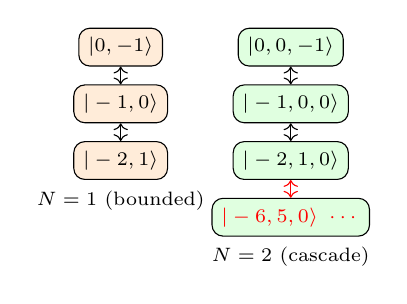
\begin{tikzpicture}[scale=0.72,every node/.style={font=\scriptsize}]
        \node[draw,rounded corners,fill=orange!15] (a) at (0,0) {$|0,-1\rangle$};
        \node[draw,rounded corners,fill=orange!15] (b) at (0,-1) {$|-1,0\rangle$};
        \node[draw,rounded corners,fill=orange!15] (c) at (0,-2) {$|-2,1\rangle$};
        \draw[<->] (a)--(b); \draw[<->] (b)--(c);
        \node at (0,-2.7) {$N=1$ (bounded)};
        \node[draw,rounded corners,fill=green!12] (x) at (3,0) {$|0,0,-1\rangle$};
        \node[draw,rounded corners,fill=green!12] (y) at (3,-1) {$|-1,0,0\rangle$};
        \node[draw,rounded corners,fill=green!12] (z) at (3,-2) {$|-2,1,0\rangle$};
        \node[draw,rounded corners,fill=green!12,text=red] (w) at (3,-3) {$|-6,5,0\rangle\ \cdots$};
        \draw[<->] (x)--(y); \draw[<->] (y)--(z); \draw[<->,red] (z)--(w);
        \node at (3,-3.7) {$N=2$ (cascade)};
      \end{tikzpicture}
    \end{column}
  \end{columns}
  \source{\refJTb}
\end{frame}

\begin{frame}{Two-molecule polaritonic spectrum (reproduced)}
  \begin{columns}[T]
    \begin{column}{0.6\textwidth}
      \centering
      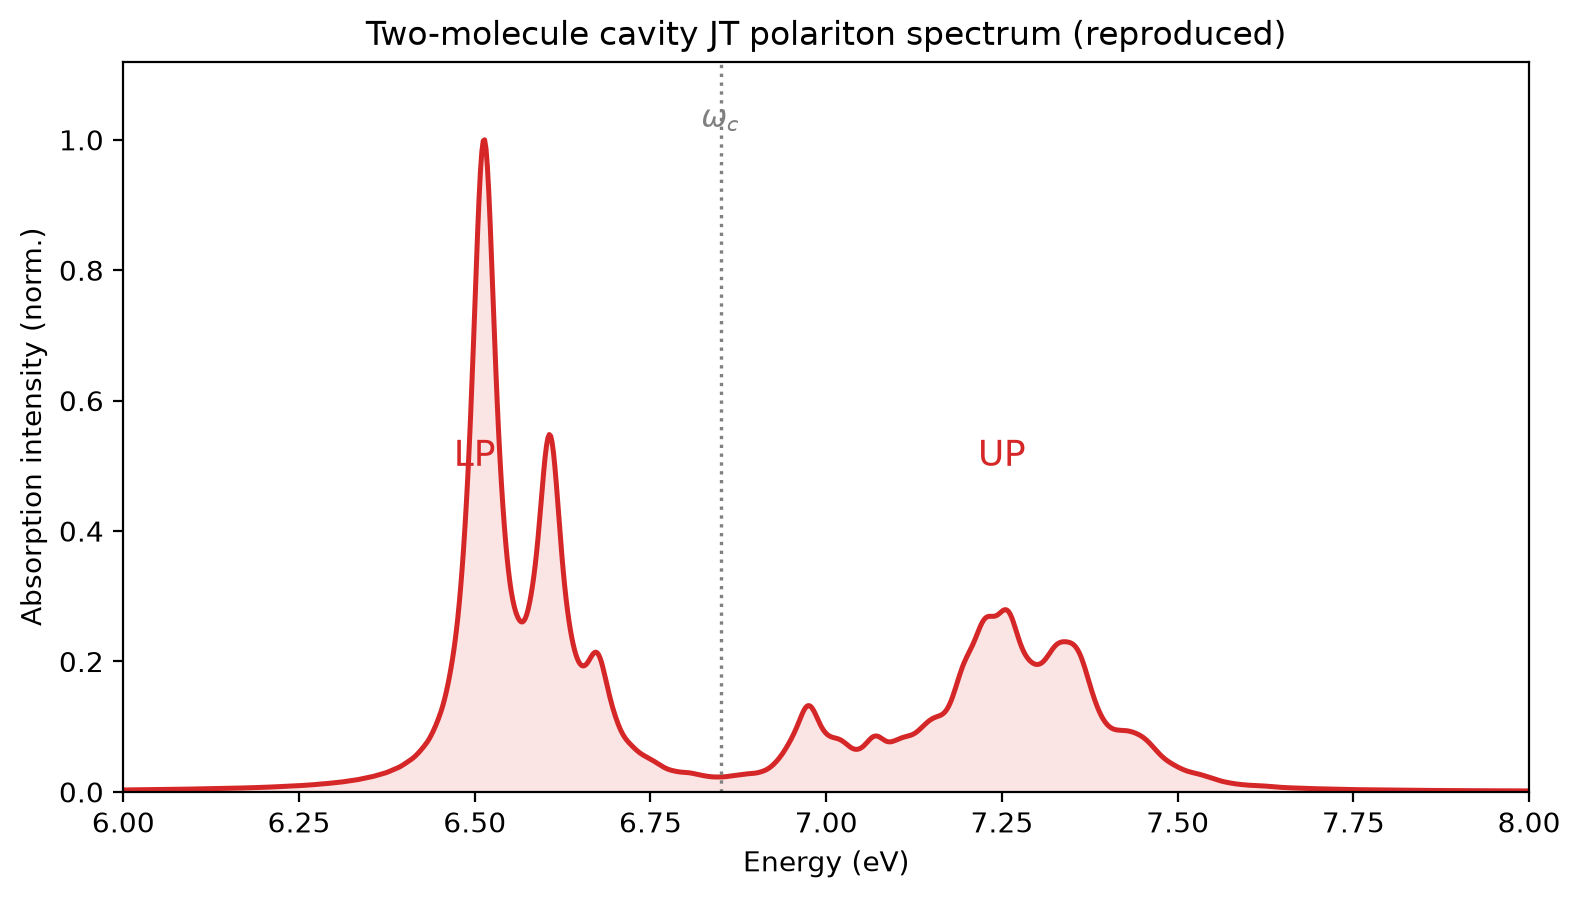
\includegraphics[width=\linewidth]{fig_repro_2mol.png}
    \end{column}
    \begin{column}{0.4\textwidth}
      \small
      \begin{itemize}
        \item LP branch stays fairly sharp; \textbf{UP branch broadens} into
              many short stems --- the cascade fingerprint.
        \item $N=2$ reaches $\mathrm{PR}$ up to $\sim 20$ (vs $\le 3$ for
              $N=1$).
        \item Broadening grows with $N$; photon-polarization dynamics get
              suppressed.
      \end{itemize}
      \vspace{0.4em}
      {\scriptsize We reproduce the $N=2$ spectrum and the vibronic-sector
      heatmap (next section) of the paper.}
    \end{column}
  \end{columns}
  \source{Physics: \refJTb\ \ Spectrum reproduced with our code.}
\end{frame}

\begin{frame}{Vibronic-sector heatmap $P(v)$ --- clean $N=2$ (reproduced)}
  \begin{columns}[T]
    \begin{column}{0.62\textwidth}
      \centering
      \includegraphics[width=\linewidth]{heatmap_figS1_Nv12.png}
    \end{column}
    \begin{column}{0.38\textwidth}
      \small
      For every \emph{bright} polaritonic eigenstate we plot the probability
      $P(v)$ that a molecule occupies vibronic sector $v$:
      \[P^{(k)}(v_0)=\!\!\sum_{a:\,v_a=v_0}\sum_{b,p}|C_{a,b,p}|^2\]
      \begin{itemize}\scriptsize
        \item x: bright states (energy-ordered); y: sector $v$; color: $P(v)$.
        \item Clean $N=2$: \textbf{42 bright states}, $\mathrm{PR}_{\max}\approx20$,
              $v\in[-15,14]$.
        \item This is the paper's Fig.~S1 --- our reference baseline.
      \end{itemize}
    \end{column}
  \end{columns}
  \source{Fig.~S1 of \refJTb\ \ Reproduced with our code.}
\end{frame}

%=============================================================================
\section{Introducing disorder}
%=============================================================================
\begin{frame}{Why disorder? Two guiding papers}
  \small
  Real molecular ensembles are \textbf{inhomogeneous}: each molecule has a
  slightly different transition energy (static \emph{energy disorder}). Two
  works frame what disorder does to a cavity-coupled ensemble:
  \begin{block}{(a) Arrowhead-matrix picture (single excitation)}
  \scriptsize
  In the single-excitation sector the disordered Tavis--Cummings Hamiltonian is
  an \textbf{arrowhead matrix}: a disordered diagonal of molecular energies plus
  one coupling row/column to the photon. Its eigenstates are two
  \textbf{polariton outliers} (split by $\pm\sqrt N g$) plus $N-1$
  \textbf{dark states}; disorder induces \emph{semi-localization} and reshapes
  the photon spectral function.
  \end{block}
  \begin{block}{(b) Disordered Holstein--Tavis--Cummings (with vibrations)}
  \scriptsize
  Adds vibrations (Holstein coupling). Central result: \textbf{disorder
  enhances} excitation transfer and vibrational entanglement, and dark states
  \emph{acquire photon weight} (brighten). Effect peaks when disorder
  $W\sim g_c$.
  \end{block}
  \source{(a) \refArrow\quad (b) \refWell}
\end{frame}

\begin{frame}{Disorder: the equations}
  \small
  \textbf{Disordered Holstein--Tavis--Cummings model} (Wellnitz \textit{et al.}):
  \[
    \hat H=\hat H_{\mathrm{TC}}+\hat H_{\mathrm{vib}}+\hat H_{\mathrm{H}}+\hat H_{\mathrm{dis}},
    \qquad
    \boxed{\ \hat H_{\mathrm{dis}}=\sum_n \epsilon_n\,\hat\sigma_n^+\hat\sigma_n^-\ }
  \]
  with i.i.d.\ energy offsets $\epsilon_n$ of mean $0$ and variance $W^2$
  (Gaussian). Consequences quantified in the papers:
  \begin{columns}[T]
    \begin{column}{0.5\textwidth}
      \begin{itemize}\scriptsize
        \item Dark states gain photon weight
              $\sum_{\mathrm{dark}}|\langle d|1_{\mathrm{ph}}\rangle|^2\approx W^2/2g_c^2$
              $\Rightarrow$ they \textbf{appear in absorption}.
        \item Polaritons stay protected while $g$ beats disorder: crossover at
              $W\sim 2g$.
      \end{itemize}
    \end{column}
    \begin{column}{0.5\textwidth}
      \begin{itemize}\scriptsize
        \item Arrowhead: photon spectral function
              $A(\varepsilon)=\sum_a \mathrm{PW}_a\,\delta(\varepsilon-\varepsilon_a)$
              --- this \emph{is} the absorption spectrum.
        \item Eigenstate amplitudes $\psi_{a,j}\sim 1/(\varepsilon_a-\omega_j)^2$;
              level statistics Poisson $\to$ semi-Poisson.
      \end{itemize}
    \end{column}
  \end{columns}
  \begin{alertblock}{Caveat}
  \scriptsize These results are for the large-$N$ ($N\to\infty$) limit. We study
  the \textbf{$N=2$ analog} --- so we use them as the conceptual framework, not
  as claims of multifractality at $N=2$.
  \end{alertblock}
  \source{\refWell\ (HTC, $\hat H_{\mathrm{dis}}$, $W^2/2g_c^2$);\ \ \refArrow\ ($A(\varepsilon)$, statistics).}
\end{frame}

%=============================================================================
\section{Disorder in our model \& results}
%=============================================================================
\begin{frame}{How disorder enters our model}
  \small
  We add \textbf{Gaussian site-energy disorder} to the two JT molecules'
  transition energies:
  \[
    \epsilon_i \sim \mathcal N(\epsilon,\ \sigma^2),\qquad i=1,2,\qquad \epsilon=7.0~\text{eV}.
  \]
  Per disorder \emph{realization} we build $\hat H$ in the
  $(n_{\mathrm{ex}}=1,\ j=-1)$ sector, diagonalize, take the intensity of each
  eigenstate as $|\langle i_0|\psi\rangle|^2$ (overlap with the ground state $+$
  one photon), broaden with a Lorentzian (FWHM $\gamma=0.044$~eV), and
  \textbf{average over realizations}.
  \begin{block}{Energy scales (from \texttt{spectrum/config.py})}
  \centering\scriptsize
  \begin{tabular}{lll}
    \toprule
    vibrational quantum $\omega$ & $0.082$~eV & JT coupling $\kappa/\omega=2.2$\\
    per-molecule coupling $g=\Omega/2\sqrt N$ & $0.242$~eV & cavity $\omega_c=6.85$~eV\\
    Rabi splitting $\Omega=2\sqrt N g$ & $0.685$~eV & sites $\epsilon=7.0$~eV, $N=2$\\
    \bottomrule
  \end{tabular}
  \end{block}
  Disorder strength quoted relative to $g$: we run at $\sigma\approx 2g$
  (strong-disorder band), where the representative cases are physically distinct.
  \ourcode
\end{frame}

\begin{frame}{Disorder realizations: the Gaussian distribution}
  \begin{columns}[T]
    \begin{column}{0.62\textwidth}
      \centering
      \includegraphics[width=\linewidth]{disorder_gaussian_sigma0.48.png}
    \end{column}
    \begin{column}{0.38\textwidth}
      \small
      \begin{itemize}
        \item Each molecule's site energy is drawn from
              $\mathcal N(\epsilon,\sigma^2)$ with $\sigma=0.48$~eV.
        \item $\sigma/g\approx 2.0$, $\sigma/\Omega\approx 0.70$ --- just below
              the $W=2g$ crossover.
        \item Dashed lines / arrow mark $\pm\sigma$ ($-0.48$ to $+0.48$~eV).
        \item We average absorption over 100 such realizations.
      \end{itemize}
    \end{column}
  \end{columns}
  \source{Disorder-strength choice motivated by \refWell / \refArrow.\ \ Plot: our code.}
\end{frame}

\begin{frame}{Representative-realization analysis: the $(\epsilon_1,\epsilon_2)$ cloud}
  \begin{columns}[T]
    \begin{column}{0.56\textwidth}
      \centering
      \includegraphics[width=\linewidth]{representative_scatter_Nv12_sigma0.48.png}
    \end{column}
    \begin{column}{0.44\textwidth}
      \small
      Behind the disorder average lie many individual $(\epsilon_1,\epsilon_2)$
      draws. We pick \textbf{9 physically meaningful realizations} (Cases
      A--I), each best satisfying a criterion on the actual drawn energies:
      \begin{itemize}\scriptsize
        \item common-mode shift $s=(\delta_1+\delta_2)/2$ vs.\ $\sqrt N g$;
        \item inter-molecular mismatch $\Delta=\epsilon_1-\epsilon_2$ vs.\ $g$.
      \end{itemize}
      \vspace{0.3em}
      Dotted lines mark $\omega_c$; the ``$+$'' marks the clean $(\epsilon,\epsilon)$.
      Each case is then recomputed individually.
    \end{column}
  \end{columns}
  \ourcode
\end{frame}

\begin{frame}{The nine representative cases ($\sigma=0.48$~eV)}
  \centering\scriptsize
  \begin{tabular}{cllccc}
    \toprule
    Case & Description & $(\epsilon_1,\epsilon_2)$ & $\Delta$ & \#bright & verdict\\
    \midrule
    A & Resonant baseline (no disorder) & (6.98, 7.01) & $0.02$ & 39 & $\approx$ clean\\
    B & Mismatch $\approx$ coupling & (7.13, 7.37) & $g$ & 14 & partial\\
    C & Large mismatch (localized) & (8.08, 7.08) & $4g$ & 11 & \textbf{dead}\\
    D & Opposite disorder & (6.28, 7.76) & $6g$ & 14 & partial$\to$dead\\
    E & Common blue detuning & (7.33, 7.17) & $0.17$ & 12 & partial\\
    F & Common red (matched) & (6.67, 6.70) & $0.03$ & \textbf{104} & \textbf{enhanced}\\
    G & Single-molecule resonant & (7.01, 6.75) & $g$ & \textbf{132} & \textbf{enhanced}\\
    H & Bare-molecule limit & (6.25, 6.15) & $0.10$ & 8 & \textbf{dead}\\
    I & A--D line, closest to $\omega_c$ & (6.72, 7.33) & $2.5g$ & 46 & intermediate\\
    \bottomrule
  \end{tabular}
  \vspace{0.6em}
  \par\raggedright\footnotesize
  \#bright $=$ number of bright vibronic (polaritonic) states above $1\%$ of the
  peak. Clean $N=2$ reference: \textbf{42}. Disorder can \emph{brighten} dark
  states (F, G, I $>$ 42/39) or kill the cascade (C, H).
  \ourcode
\end{frame}

\begin{frame}{Case spectra: baseline vs.\ A--D line}
  \begin{columns}[T]
    \begin{column}{0.5\textwidth}
      \centering
      \includegraphics[width=\linewidth]{representative_spectrum_Nv12_sigma0.48_caseA.png}\\
      {\scriptsize \textbf{Case A} --- near-zero disorder reproduces the clean
      collective cascade.}
    \end{column}
    \begin{column}{0.5\textwidth}
      \centering
      \includegraphics[width=\linewidth]{representative_spectrum_Nv12_sigma0.48_caseI.png}\\
      {\scriptsize \textbf{Case I} --- interior point on the A--D line: broad,
      spread oscillator strength, brightest near $\omega_c$.}
    \end{column}
  \end{columns}
  \vspace{0.3em}
  \centering\footnotesize
  Cascade weakens monotonically along the A--D line:
  $\mathrm{PR}\ 20.6\ (\mathrm{A})\to 16.2\ (\mathrm{I})\to 8.5\ (\mathrm{D})$ as
  opposite-disorder mismatch grows.
  \ourcode
\end{frame}

\begin{frame}{Heatmap analysis with LP/UP energy axis}
  \begin{columns}[T]
    \begin{column}{0.62\textwidth}
      \centering
      \includegraphics[width=\linewidth]{representative_heatmap_Nv12_sigma0.48_caseI.png}
    \end{column}
    \begin{column}{0.38\textwidth}
      \small
      \begin{itemize}
        \item Left y-axis: vibronic sector $v$; color: $P(v)$.
        \item Right y-axis (red): each bright state's \textbf{energy} vs.\ the
              same index --- a \emph{jump} marks the LP$\to$UP branch boundary.
        \item Case I: \textbf{46 bright states}, $\mathrm{PR}_{\max}=16.2$,
              $v\in[-14,13]$.
        \item Opposite disorder \emph{brightens} dark states (46 $>$ 39 at A)
              yet lowers per-state spread.
      \end{itemize}
    \end{column}
  \end{columns}
  \source{$P(v)$ heatmap def.\ from Fig.~S1 of \refJTb.\ \ Energy-axis overlay \& computation: our code.}
\end{frame}

\begin{frame}{Number of bright vibronic states vs.\ case}
  \begin{columns}[T]
    \begin{column}{0.55\textwidth}
      \centering
      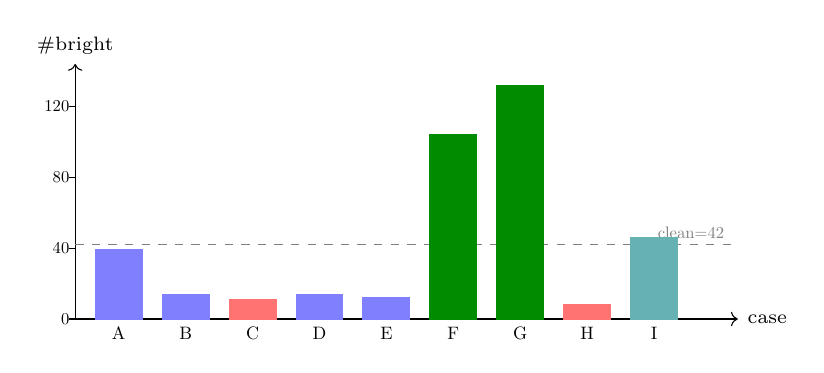
\begin{tikzpicture}[yscale=0.9,xscale=0.85]
        % y-axis (scaled: 1 unit = 40 bright states), max 132 -> 3.3
        \draw[->] (-0.3,0)--(9.6,0) node[right]{\scriptsize case};
        \draw[->] (-0.3,0)--(-0.3,3.6) node[above]{\scriptsize \#bright};
        \draw (-0.4,0)--(-0.3,0) node[left,scale=0.6]{0};
        \draw (-0.4,1)--(-0.3,1) node[left,scale=0.6]{40};
        \draw (-0.4,2)--(-0.3,2) node[left,scale=0.6]{80};
        \draw (-0.4,3)--(-0.3,3) node[left,scale=0.6]{120};
        % reference line at 42 -> 1.05
        \draw[dashed,gray] (-0.3,1.05) -- (9.5,1.05);
        \node[gray,scale=0.6] at (8.9,1.22){clean=42};
        % bars: value/40 gives height
        \filldraw[blue!50]        (0,0) rectangle (0.7,0.975);  % A 39
        \filldraw[blue!50]        (1,0) rectangle (1.7,0.35);   % B 14
        \filldraw[red!55]         (2,0) rectangle (2.7,0.275);  % C 11
        \filldraw[blue!50]        (3,0) rectangle (3.7,0.35);   % D 14
        \filldraw[blue!50]        (4,0) rectangle (4.7,0.30);   % E 12
        \filldraw[green!55!black] (5,0) rectangle (5.7,2.60);   % F 104
        \filldraw[green!55!black] (6,0) rectangle (6.7,3.30);   % G 132
        \filldraw[red!55]         (7,0) rectangle (7.7,0.20);   % H 8
        \filldraw[teal!60]        (8,0) rectangle (8.7,1.15);   % I 46
        \foreach \x/\l in {0/A,1/B,2/C,3/D,4/E,5/F,6/G,7/H,8/I}
          {\node[scale=0.65] at (\x+0.35,-0.2){\l};}
      \end{tikzpicture}
    \end{column}
    \begin{column}{0.45\textwidth}
      \small
      \begin{itemize}
        \item \textcolor{green!55!black}{\textbf{Enhanced}} (F, G): matched /
              single-resonant $\Rightarrow$ disorder brightens the whole dark
              manifold ($104$, $132\gg42$).
        \item \textcolor{teal!60}{\textbf{Intermediate}} (I): opposite disorder
              on the A--D line ($46$).
        \item \textcolor{blue!50}{\textbf{Partial}} (A, B, D, E).
        \item \textcolor{red!55}{\textbf{Dead}} (C, H): localization /
              decoupling collapse the cascade ($\le 11$).
      \end{itemize}
    \end{column}
  \end{columns}
  \ourcode
\end{frame}

%=============================================================================
\section*{Summary}
%=============================================================================
\begin{frame}{Summary}
  \small
  \begin{enumerate}
    \item \textbf{Reproduced} the single-molecule cavity-JT polariton spectrum
          (LP/UP, bounded $v$) and the two-molecule collective spectrum +
          $P(v)$ heatmap (unbounded cascade, $\mathrm{PR}\sim20$).
    \item \textbf{Introduced disorder} following the arrowhead-matrix and
          disordered Holstein--Tavis--Cummings frameworks: Gaussian site-energy
          disorder $\epsilon_i\sim\mathcal N(\epsilon,\sigma^2)$, dark states
          brighten, cascade protected while $g$ beats $\sigma$.
    \item \textbf{Implemented \& analyzed} disorder in our $N=2$ model:
          realizations, representative cases (A--I), and $P(v)$ heatmaps with an
          LP/UP energy overlay.
    \item \textbf{Key result:} the number of bright vibronic states and the
          cascade PR track the two disorder axes --- \emph{enhanced} (F, G, I),
          \emph{partial}, or \emph{dead} (C, H).
  \end{enumerate}
  \vspace{0.4em}
  \centering\footnotesize Outlook: larger $N$, LP/UP-resolved PR correlation,
  stronger disorder ($\sigma\sim10g$) to test cascade survival.
\end{frame}

\begin{frame}{References}
  \footnotesize
  \begin{enumerate}
    \item \refJTa
    \item \refJTb
    \item \refArrow
    \item \refWell
    \item \refJahn
    \item \refEbbesen
  \end{enumerate}
\end{frame}

\end{document}
